%% Part A
%% article:文档类型
%% 11pt:字体
\documentclass[11pt]{article}

%% Part B(包) 
\usepackage{fullpage}  
\usepackage{graphicx}
\usepackage{amssymb}
\usepackage{fancyvrb}
\usepackage{listings} 
\usepackage{xcolor}
\usepackage{fontspec, xunicode, xltxtra, graphicx, subfig}
\usepackage{amsmath}
\usepackage{indentfirst}
\usepackage{xeCJK} 
\setlength{\parindent}{2em}
\setmainfont{Times New Roman}  
\setCJKmainfont{Songti SC}
\newfontfamily\monaco{Monaco}
\definecolor{backcolour}{rgb}{0.95,0.95,0.92}
%% Part C(代码样式)
\lstset{keywordstyle=\color{blue}, %%设置关键字颜色  
        commentstyle=\color[cmyk]{1,0,1,0}, %% 设置注释颜色  
        backgroundcolor=\color{backcolour}, %% 设置边框格式  
        escapeinside=``, %% 逃逸字符(1左面的键),用于显示中文  
        extendedchars=false, %% 解决代码跨页时,章节标题,页眉等汉字不显示的问题  
        xleftmargin=2em,xrightmargin=2em, aboveskip=1em, %% 设置边距   
        showspaces=false, %% 不显示空格  
        tabsize=4, %% 设置tab空格数 
        breaklines,
        numbers=left, numberstyle=\tiny,
        basicstyle=\small\monaco
       } 
 
%% Part D(正文)
\begin{document}

%\begin{CJK}{UTF8}{song} %% 使用中文 song为宋体
 
\title{统计计算第三次作业}  
\author{吕坤升, 15338140, 统计学}
\date{\today}
\maketitle
\tableofcontents

\section{Please write down the form of Monte Carlo average of log-likelihood (which you are
going to evaluate).}

\centerline{\textbf{Complete-data likelihood function}}

\begin{align*}
L(\Omega | Y_{ij},U_i,Z_{1,i},Z_{2,i}) &= \prod_{i=1}^{n}\prod_{c=1}^{2}\left\{\pi_cf_c(Z_{c,i})[\prod_{j=1}^T f_c(Y_{ij}|Z_{c,i})] \right\}^{\omega_{ic}} \\
&= exp \Bigg\{ \sum_{i=1}^n\sum_{c=1}^2\omega_{ic}\Big[ln\pi_c-ln(\sqrt{2\pi}\sigma_c)-\frac{Z_{c,i}^2}{2\sigma_c^2}+\sum_{j=1}^T[Y_{ij}lnP^{(c)}_{ij}+(1-Y_{ij})ln(1-P^{(c)}_{ij})]\Big]\Bigg\} 
\end{align*}

\centerline{\textbf{Complete-data loglikelihood function}}
\begin{align*}
l=\sum_{i=1}^n\sum_{c=1}^2\omega_{ic}\Big[ln\pi_c-ln(\sqrt{2\pi}\sigma_c)-\frac{Z_{c,i}^2}{2\sigma_c^2}+\sum_{j=1}^T[Y_{ij}lnP^{(c)}_{ij}+(1-Y_{ij})ln(1-P^{(c)}_{ij})]\Big]
\end{align*}


$l$中的$Z_1,Z_2,U$为missing data,在后面的代码中不再单独分开$Z1$和$Z2$,可以看成$Z=I_{U=1}Z_1+I_{U=2}Z2$。设置$\Omega=(\beta_1,\beta_2,\sigma_1,\sigma_2,\pi_1)$

这里用MCEM方法要优化的蒙特卡洛log似然函数均值为:$$Q(\Omega|\Omega^{m})=E(l|Y_{ij},\Omega^{(m)})=\frac{1}{N}\sum_{k=1}^{N} \sum_{i=1}^n\sum_{c=1}^2\omega_{ic}\Big[ln\pi_c-ln(\sqrt{2\pi}\sigma_c)-\frac{Z_{i,k}^2}{2\sigma_c^2}+\sum_{j=1}^T[Y_{ij}lnP^{(c)}_{ij}+(1-Y_{ij})ln(1-P^{(c)}_{ij})]\Big].$$ 其中的$Z_{i,k}$和对应的$U_i$是从条件分布$p(U,Z|Y_{ij},\Omega^{(m)})$中抽取的。

\section{Please write down details of the EM algorithm you use for this simulation, especially
the Metropolis-Hastings steps.}



为了从条件分布$p(U,Z|Y_{ij},\Omega^{(m)})$中抽取missing data U和Z,注意到这里的U和Z都是100维(n维)的,且每一维对应的$X_{c,ij},Y_{ij}$都不一样,因此对于U和Z的每一维都需要单独的抽样。对于每一维,我们先给定初值$U^{(0)}$和$Z^{(0)}$,利用$P(U^{(k+1)}|Y_{ij},Z^{(k)},\Omega^{(m)})$确定U的第k+1维,再利用$P(Z^{(k+1)}|Y_{ij},U^{(k+1)},\Omega)$来确定Z的第k+1维。在这里注意,U的条件分布可以写出显性表达式且容易得到取1或2的概率,可以直接算出概率利用伯努利分布来直接抽样,但Z的条件分布十分难求,因此对Z的每一维都需要用到Metropolis-Hasting method。

具体的EM算法如下:

\centerline{\textbf{E-Step}}

\centerline{\textbf{第m步时}}

\centerline{\textbf{Gibbs Sampling}}
在这里我们需要从条件分布$p(U,Z|Y_{ij},\Omega^{(m)})$中抽取$N_{Gibbs}$份Z和U。

对于每一份的抽取:

\begin{itemize}
  \centerline{\textbf{给定第k-1维的Z($Z^{(k-1)}$)}}
  
  \item 1) 计算$$p_1=\pi_1^{(m)}\frac{1}{\sqrt{2\pi}\sigma_1^{(m)}}e^{-\frac{(Z^{(k-1)})^2}{2(\sigma_1^{(m)})^2}}\prod_{j=1}^{T}(P^{(1)}_{ij})^{Y_{ij}}(1-P^{(1)}_{ij})^{1-Y_{ij}}.$$ 
  \item 2) 计算$$p_2=\pi_2^{(m)}\frac{1}{\sqrt{2\pi}\sigma_2^{(m)}}e^{-\frac{(Z^{(k-1)})^2}{2(\sigma_2^{(m)})^2}}\prod_{j=1}^{T}(P^{(2)}_{ij})^{Y_{ij}}(1-P^{(2)}_{ij})^{1-Y_{ij}}.$$ 其中$P^{(c)}_{ij}=g^{-1}(\beta_c X_{c,ij} + Z^{(k-1)})$. 
  \item 3) 因为$P(U^{(k+1)}=1|Y_{ij},Z^{(k)},\Omega^{(m)})$和$P(U^{(k+1)}=2|Y_{ij},Z^{(k)},\Omega^{(m)})$的分母相同,因此只需计算分子($p_1 \& p_2$),找到归一化参数,则可以得到$p = P(U^{(k+1)}=1|Y_{ij},Z^{(k)},\Omega^{(m)})=\frac{p_1}{p_1+p_2}$.
  \item 4) 用伯努利分布进行抽样,第k维的U($U^{(k)}$)以$p$为概率取1,以1-$p$的概率取2.
  \par
  \centerline{\textbf{给定第k维的U($U^{(k)}$)}}
  \centerline{\textbf{Metropolis-Hasting Method}}
  \item 1) 给定马氏链的第t个元素,记为$Z_t$,以$N(Z_t,1)$的转移概率抽取下一个元素$y$
  \item 2) 
  \subitem 若$U^{(k)}$为1,则计算$$p_{up}=\frac{1}{\sqrt{2\pi}\sigma_1^{(m)}}e^{-\frac{y^2}{2(\sigma_1^{(m)})^2}}\prod_{j=1}^{T}(P^{(1)}_{ij})^{Y_{ij}}(1-P^{(1)}_{ij})^{1-Y_{ij}},$$ $$p_{under}=\frac{1}{\sqrt{2\pi}\sigma_1^{(m)}}e^{-\frac{Z_t^2}{2(\sigma_1^{(m)})^2}}\prod_{j=1}^{T}(P^{(1)}_{ij})^{Y_{ij}}(1-P^{(1)}_{ij})^{1-Y_{ij}},$$ 
  \subitem 若$U^{(k)}$为2,则计算$$p_{up}=\frac{1}{\sqrt{2\pi}\sigma_2^{(m)}}e^{-\frac{y^2}{2(\sigma_2^{(m)})^2}}\prod_{j=1}^{T}(P^{(2)}_{ij})^{Y_{ij}}(1-P^{(2)}_{ij})^{1-Y_{ij}},$$ $$p_{under}=\frac{1}{\sqrt{2\pi}\sigma_2^{(m)}}e^{-\frac{Z_t^2}{2(\sigma_2^{(m)})^2}}\prod_{j=1}^{T}(P^{(2)}_{ij})^{Y_{ij}}(1-P^{(2)}_{ij})^{1-Y_{ij}}.$$ 
  \item 3) 计算 $$p=\frac{p_{up}}{p_{under}}.$$
  \item 4) 抽取$rand\sim U(0,1)$
  \item 5) 
  \subitem 若 $rand <= p$, 马氏链的第t+1个元素$Z_{t+1}=y$
  \subitem 若 $rand > p $, 马氏链的第t+1个元素$Z_{t+1}=Z_t$
  \item 6) 重复步骤1-5,1000次,得到一条1000个元素的马氏链,丢弃前900个元素,在最后100个元素中随机抽取1个元素作为第k维的Z($Z^{(k)}$)
  %[\beta_1^{(m)}X_{1,kj}+Z^{(k-1)}] 
% \begin{align*}
%   P(U^{(k+1)}|Y_{ij},Z^{(k)},\Omega^{(m)}) 
%   &=

% \end{align*}
\end{itemize}
重复上述算法n次,可得到一份满足要求的U和Z。再重复$N_{Gibbs}$次,则可以得到进行MCEM所需的$N_{Gibbs}$份随机样本。丢弃掉前100份随机样本,作为burn-in,将剩余的随机样本代入式子,
计算期望值:
$$Q=E(l|\Omega^{(m)})=\frac{1}{N}\sum_{k=1}^{N} \sum_{i=1}^n\sum_{c=1}^2\omega_{ic}\Big[ln\pi_c-ln(\sqrt{2\pi}\sigma_c)-\frac{Z_{i,k}^2}{2\sigma_c^2}+\sum_{j=1}^T[Y_{ij}lnP^{(c)}_{ij}+(1-Y_{ij})ln(1-P^{(c)}_{ij})]\Big]$$
此时,这里的$Z_{i,k}$和对应的$U_i$,是指经历上述算法后得到的。这里的$N=N_{Gibbs}-N_{burn-in}$
% 则,在第m个2a步,挑选$\beta^{(m+1)}$最大化:
% $$E\Big[ln\Big(f_{Y|Z_1,Z_2,U}(Y|Z_1,Z_2,U,\beta_1^{(m)},\beta_2^{(m)})\Big)\Big|y\Big]$$
% 在第m个2b步,挑选$\sigma_1^{(m+1)},\sigma_2^{(m+1)},\pi_1^{(m+1)}$最大化:
% $$E\Big[ln\Big(f_{(Z_1,Z_2,U)}(Z_1,Z_2,U|\sigma_1^{(m)},\sigma_2^{(m)},\pi_1^{(m)})\Big)\Big|y\Big]$$

% 但是无法计算,因此使用MCEM,重点在于要从$f_{Z_1,Z_2,U|Y}(Z_1,Z_2,U|Y,\beta_1^{(m)},\beta_2^{(m)},\sigma_1^{(m)},\sigma_2^{(m)},\pi_1^{(m)})$中抽取500-400个$(Z_1,Z_2,U)^{(k)}$,且每一个$(Z_1,Z_2,U)^{(k)}$,都是100(n)维的。

% 在这里,可以写成$$p(U,Z_1,Z_2|Y_{ij},\Omega^{(m)})=\dfrac{P(\Omega^{(m)},U)P(Z_1,Z_2|U,\Omega^{(m)})P(Y|Z_1,Z_2,\Omega^{(m)},U)}{c}$$
% \centerline{\textbf{Gibbs sampling}}
% 已知:第m步E-step的参数$\sigma_1^{(m)},\sigma_2^{(m)},\pi_1^{(m)},\beta^{(m)}$,设定$U,Z_1,Z_2$的初值$U^{(0)},Z_1^{(0)},Z_2^{(0)}$。

% 分别从三个条件分布中抽取$U,Z_1,Z_2$:
% \begin{itemize}
%   \item $P(U^{(1)}|Z_1^{(0)},Z_2^{(0)})$,在给定$Z_1,Z_2$时,用MH抽样方法,以1-2伯努利分布作为转移概率,参数p为:上一个U为1的时候为$\pi^{(m)}$,上一个U为0的时候为$1-\pi^{(m)}$.
%   \item $P(Z_1^{1}|U^{(1)},Z_2^{(0)})$,在给定$U^{(1)},Z_2^{(0)}$时,在抽$Z_1^{(1)}$时使用MH抽样方法,用$Z_1^{0}$作为初值,因为每一个i对应的X都不一样,因此需要构造100条马氏链,分开抽每一维,这里因为转移概率相等,因此使用随机游走的MH方法较为简单,以正态分布$N(Z_{1,(i-1)},2)$作为转移的分布。
%   \item $P(Z_2^{1}|U^{(1)},Z_2^{(0)})$,在给定$U^{(1)},Z_2^{(0)}$时,在抽$Z_1^{(1)}$时使用MH抽样方法,用$Z_1^{0}$作为初值,因为每一个i对应的X都不一样,因此需要构造100条马氏链,分开抽每一维,这里因为转移概率相等,因此使用随机游走的MH方法较为简单,以正态分布$N(Z_{2,(i-1)},10)$作为转移的分布。
% \end{itemize}

% \centerline{\textbf{Metropolis-Hasting}}
% 以从$P(Z_1^{(1)}|U^{(1)},Z_2^{(0)})$中抽取$Z_1$为例:
% \begin{itemize}
%   \item 构造提议分布$N(Z_{1,(i-1)},2)$
%   \item 从提议分布中生成$Z_{1,(i)}$
%   \item 从$U(0,1)$中产生均匀分布随机数UU
%   \item 若$UU\leq \frac{f(Z_{1,(i)})}{f(Z_{1,(i-1)})}$,则接受$Z_{1,(i)}$,否则$Z_{1,(i)}=Z_{1,(i-1)}$.
%   \item i = i + 1, 返回到第三步
% \end{itemize}

% 由此可以生成第一份$U,Z_1,Z_2$,交错的更新最终得到500份这样的$U,Z_1,Z_2$,取前100份$U,Z_1,Z_2$作为burn-in,剩余的400份用来求Q。
  
\centerline{\textbf{M-Step}}
运用拟牛顿法(Quasi-Newton Methods)最大化上面好不容易得到的Q,更新新一轮的参数。
验证是否收敛,不收敛则返回到上一步。

\centerline{\textbf{Trick}}
\begin{itemize}
\item 在这里,$N=N_Gibbs-N_{burn-in}$随迭代的次数逐渐增加,在代码中设置为第m次迭代的时候,$N = 5 * m$。
\item 设置T=30,可以更快的达到收敛。
\end{itemize}

\section{What are your initial values? What is your convergence rule?}
初值设置为$$\beta_1=0.5,\beta_2=1.5,\sigma_1=2.5,\sigma_2=11,\pi_1=0.8,$$ 在100次simulation中,设置当第m次迭代更新产生的参数与上一次产生的参数差距小于0.1定为收敛,在一次simulation中,设置差距小于0.01才收敛,但在跑最大次数前仍然无法收敛,但是从Figure 1中可看出来已经是收敛了。

\section{How to accelerate your EM algorithm? Any improvement you can observe?}
\begin{itemize}
  \item 拟牛顿法因为不需要二阶导数的信息,比普通的牛顿法更加有效。在这里使用了拟牛顿法。
  \item 在R中使用sapply而不是for作为循环,然后可使用snowfall等Rpackage进行并行。
  \item 由于R中反复调用函数会降低速度,且算法中包含了大量的循环,因此将函数改成内联的形式可以大大加快代码运行的速度。使用这个方法几乎比原来耗的时间少了一半。
  \item 在M步中,一些参数可以直接写出表达式直接求导最优化,可以减少利用拟牛顿法优化的参数个数,提高速度。
\end{itemize}

\section{Try different numbers of simulations: 200,300,...,1000. And plot the corresponding
MSE.}
取了一次simulation的结果,Figure 1 画出每个参数的update path,可以看到除了$\sigma_2$的估计较为不准外,其他参数与参数差距较小。
\begin{figure}[htbp]%%图  
    \centering  %插入的图片居中表示  
    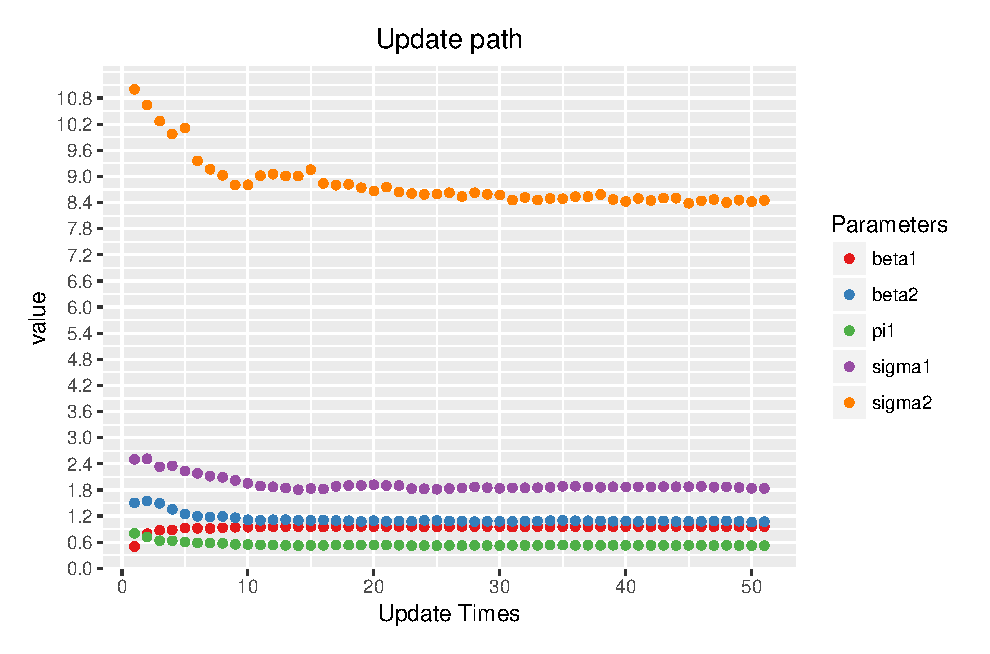
\includegraphics[scale=0.8]{update_path.eps}   
    \caption{Update path of five parameters for single simulation.}  %图片的名称  
    \label{update}   %标签,用作引用  
\end{figure}  



由于simulation跑的十分的慢,即使放松了收敛的条件,在作业截止时间前最多跑了17次,将每一次的MSE依次数画成散点图,如Figure 2,可以观察到每一次的MSE保持大致的稳定。

\begin{figure}[htbp]%%图  
    \centering  %插入的图片居中表示  
    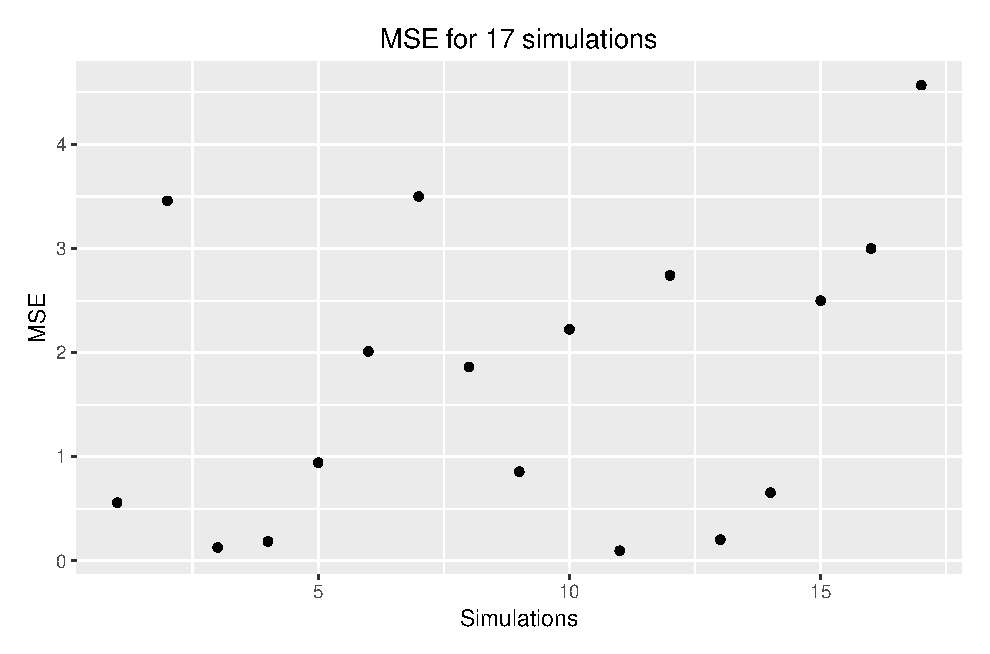
\includegraphics[scale=0.8]{MSE.eps}   
    \caption{MSE for 17 simulations.}  %图片的名称  
    \label{MSE}   %标签,用作引用  
\end{figure} 


% 考虑将$Z_1,Z_2$ 合并成一个 $Z_i=Z_{(1i)}*I_{(U_i=1)}+Z_{2i}*I_{(U_i=2)}$,此时$Z\sim \Phi_1*I_{(U_i=1)}+\Phi_2*I_{(U_i=2)}$。

% \centerline{\textbf{Metropolis}}
% $$P(Z|U,Y,\Omega^{[t]})=\dfrac{P(Z,U,Y,\Omega^{[t]})}{\int P(Z,U,Y,\Omega^{[t]}) dZ}$$
% 这个密度函数求不出来,因此随机数只能通过MH算法来得到了。

% $$P(U|Z,Y,\Omega^{[t]})=\dfrac{P(Z,U,Y,\Omega^{[t]})}{\int P(Z,U,Y,\Omega^{[t]}) dU}$$
% 这个密度函数虽然也求不出来,但是因为U只有两个取值,而且U是伯努利分布,因此可以直接代入似然函数中,得到两个与概率成正比的常数$c_1,c_2$,再找到归一化的常数$\alpha$使得$\alpha(c_1+c_2)=1$.
% 这样我们可以得到条件伯努利分布的是第一组的概率$p_1=\alpha c_1$,这样我们可以直接通过这个伯努利分布来生成随机数。


% 先给定初值$\Omega^{(0)}=\{\beta_1^{(0)},\beta_2^{(0)},\sigma_1^{(0)},\sigma_2^{(0)},\pi_1^{(0)}\}$, 此时Q可用蒙特卡洛EM方法近似,因此优化目标为:

% \begin{align*}
% Q_1(\Omega)=E(l|\Omega)=\frac{1}{N}\sum_{k=1}^Nl(Y,(U^{(k)},Z_1^{(k)},Z_2^{(k)})|\Omega^{[0]}) 
% \end{align*}

% $$(U^{(i)},Z_1^{(i)},Z_2^{(i)})\sim U,Z_1,Z_2|Y,\Omega^{(t)}$$

% 接下来应该用Gibbs Sampling Method从$U,Z_1,Z_2|Y,\Omega^{(t)}$抽取二维的样本$(U^{(i)},Z^{(i)})$

\newpage
\section{Code}
\subsection{functions}
\begin{lstlisting}[language=R] 
rm(list = ls())
setwd("C:/Users/Administrator/Desktop/lvksh/统计计算")
g <- function(x){
  return(exp(x)/(1+exp(x)))
}
logLikelihood <- function(Z, 
                          U,
                          Omega,
                          m = 1) {
  # 该函数传入100维的Z和U,计算loglikelihood
  wi1 <- which(U == 1)
  wi2 <- which(U == 2)
  
  l1 <- sapply(wi1,function(i){
    TT <- sapply(1:Time,function(j){
      eta <- Omega[1] * X1[i,j] + Z[i]
      if(eta >= 600) eta <- 600 # 限制可能出现的超大数
      TTT <- Y_ij[i,j] * (eta - log(1 + exp(eta))) + (1 - Y_ij[i,j]) * (- log(1 + exp(eta)))
      return(TTT)
    })
    lll <- (log(Omega[5]) - log(sqrt(2*pi) * Omega[3]) - Z[i]^2/(2*Omega[3]^2) + sum(TT))
    return(lll)
  })
  l1 <- sum(l1)
  
  l2 <- sapply(wi2,function(i){
    TT <- sapply(1:Time,function(j){
      eta <- Omega[2] * X2[i,j] + Z[i]
      
      if(eta >= 600) eta <- 600
      TTT <- Y_ij[i,j] * (eta - log(1 + exp(eta))) + (1 - Y_ij[i,j]) * (- log(1 + exp(eta)))
      return(TTT)
    })
    lll <- (log(1-Omega[5]) - log(sqrt(2*pi) * Omega[4]) - Z[i]^2/(2*Omega[4]^2) + sum(TT))
    return(lll)
  })
  l2 <- sum(l2)
  
  L <- l1 + l2
  return(L)
}





Gibbs_Sampling <- function(Z, # 给定初值
                           Omega,
                           m ){ # EM算法的第m步
  # 返回Gibbs抽样得到的Z,U
  # 建立存放Gibbs抽样的结果矩阵
  Z_ <- list(Z = array(dim = c(n,Gibbs_N+burn_in+1)), U = array(dim = c(n,Gibbs_N+burn_in+1)))
  # 给定初值
  Z_$Z[,1] <- Z$Z
  Z_$U[,1] <- Z$U
  # 开始交错更新
  for (k in 2:(Gibbs_N+burn_in+1))  {
      for (i in 1:n){
        # 在第k份的第i维 先生成第k份的U的第i维,再用这个用MH去抽第k份的Z的第i维
        U_Z <- Z_$Z[i,k-1]
        U_U <- Z_$U[i,k-1]
        p1 <- prod(g(Omega[1] * X1[i,] + U_Z)^Y_ij[i,] * (1 - g(Omega[1] * X1[i,] + U_Z))^(1 - Y_ij[i,])) * Omega[5] * dnorm(x = U_Z,mean = 0,sd = Omega[3]) 
        p2 <- prod( g(Omega[2] * X2[i,] + U_Z)^Y_ij[i,]  * (1 - g(Omega[2] * X2[i,] + U_Z))^(1 - Y_ij[i,])) * (1 - Omega[5]) * dnorm(x = U_Z,mean = 0,sd = Omega[4])
        prod <- p1 / (p1 + p2)
        if(is.nan(prod)) prod = 1
        Z_$U[i,k] <- rbinom(n = 1,size = 1,prob = 1 - prod) + 1
        
        # 用上面抽到的U的第i维,来抽Z的第i维,这里需要用到MH
        Z_U <- Z_$U[i,k]
        #Z_U <- Z_$Z[i,k-1]
        # 建立MH算法的马氏链
        MH_Z <- array(dim = c(1,Metro_N+1))
        MH_Z_initial <- rnorm(n = 1,mean = 0,sd = 1)
        MH_Z[1] <- MH_Z_initial # 链的第一个元素为初值
        for(t in 2:(Metro_N+1)){
          temp <- rnorm(n = 1,mean = MH_Z[t-1],sd = 1) # 以转移概率得到一个数
          if (Z_U == 1){
            p_up <- prod( (g(Omega[1] * X1[i,] + temp))^Y_ij[i,]  * (1 - g(Omega[1] * X1[i,] + temp))^(1 - Y_ij[i,])) * dnorm(x = temp,mean = 0,sd = Omega[3])
            p_under <- prod( (g(Omega[1] * X1[i,] + MH_Z[t-1]))^Y_ij[i,] * (1 - g(Omega[1] * X1[i,] + MH_Z[t-1]))^(1 - Y_ij[i,])) * dnorm(x = MH_Z[t-1],mean = 0,sd = Omega[3])
            Reject_p <- p_up / p_under
          } else if(Z_U == 2) {
            p_up <- prod( g(Omega[2] * X2[i,] + temp)^Y_ij[i,]  * (1 - g(Omega[2] * X2[i,] + temp))^(1 - Y_ij[i,])) * dnorm(x = temp,mean = 0,sd = Omega[4])
            p_under <- prod( g(Omega[2] * X2[i,] + MH_Z[t-1])^Y_ij[i,]  * (1 - g(Omega[2] * X2[i,] + MH_Z[t-1]))^(1 - Y_ij[i,])) * dnorm(x = MH_Z[t-1],mean = 0,sd = Omega[4])
            Reject_p <- p_up / p_under
          }
          rand <- runif(1)
          if(Reject_p == Inf) Reject_p <- 0.5
          if(rand <= Reject_p) MH_Z[t] <- temp
          else MH_Z[t] <- MH_Z[t-1]
        }
        Z_$Z[i,k] <- sample(x = MH_Z[(Metro_N-100):(Metro_N + 1)],size = 1)
        # 在马氏链里的最后100个数里抽一个作为最终的第k份的Z的第i维
      }
  }
  return(Z_)
}

fn <- function(Omega){
  ff <- sapply(2:(Gibbs_N + 1),function(k){
    temp <- logLikelihood(Z = Gibbs_result$Z[,burn_in +k],U = Gibbs_result$U[,burn_in +k],Omega,m)
    return(temp)
  })
  return(-mean(ff)) # 这里是负的 为了optim函数
}
  \end{lstlisting}

\subsection{Main function for 100 simulations}
  \begin{lstlisting}[language=R] 
burn_in <- 100
# initial value -----------------------------------------------------------
# Gibbs_N <- 100 #要求Gibbs的次数
reps <- 50 # 最大循环次数
Metro_N <- 1000 # 马氏链的长度
# 第一轮的参数初值
b1 <- 0.5
b2 <- 1.5
s1 <- 2.5
s2 <- 11
PI <- 0.8
Omega <- c(b1=b1,b2=b2,s1=s1,s2=s2,PI=PI)


OMEGA <- array(dim = c(5,100))
for(simulations in 1:100){
  set.seed(simulations)
  n <- 100
  Time <- 30
  beta1 <- 1
  beta2 <- 1
  pi1 <- 0.6
  sigma1 <- 2
  sigma2 <- 10
  U_i <- rbinom(n = n,size = 1,prob = 1 - pi1) + 1
  X1 <- matrix(rnorm(n = n*Time),nrow = n,ncol = Time) # fixed effect
  X2 <- matrix(rnorm(n = n*Time),nrow = n,ncol = Time)
  z1 <- rnorm(n = n,mean = 0,sd = sigma1) # random effect
  z2 <- rnorm(n = n,mean = 0,sd = sigma2)
  Y_ij <- array(dim = c(n,Time))
  for(i in 1:n) {
    for(j in 1:Time) {
      # generate the Y_ij AKA observed data
      # the group item indicates the cluster for each subject
      if(U_i[i] == 1) {
        Y_ij[i,j] <- g(beta1 * X1[i,j] + z1[i])
      }
      else {
        Y_ij[i,j] <- g(beta2 * X2[i,j] + z2[i])
      }
      Y_ij[i,j] <- rbinom(n = 1,size = 1,prob = Y_ij[i,j])
    }
  }
  
  for (m in 1:reps)  {
    Gibbs_N <- 10 * m
    U_initial <- rbinom(n = n,size = 1,prob = Omega[5]) + 1
    Z_initial <- rnorm(n = n,mean = 0,sd = (Omega[3] + Omega[4])/2)
    Z_list <- list(Z=Z_initial,U=U_initial)
    Gibbs_result <- Gibbs_Sampling(Z_list,Omega,m) 
    update_par <- optim(par = c(0.9,1.1,2.5,11,0.7),fn =  fn,method = "BFGS",control = list(trace = 2))
    update_par <- update_par$par
    if(all(abs(update_par - Omega) <= 1e-01)) {
      break
    }
    Omega <- update_par
  }
    OMEGA[,simulations] <- update_par
}
save(OMEGA,file = "OMEGA_100.rdata")
  \end{lstlisting}

\subsection{Main function for one simulation}
  \begin{lstlisting}[language=R] 
set.seed(1)
n <- 100
Time <- 10
beta1 <- 1
beta2 <- 1
pi1 <- 0.6
sigma1 <- 2
sigma2 <- 10
U_i <- rbinom(n = n,size = 1,prob = 1 - pi1) + 1
X1 <- matrix(rnorm(n = n*Time),nrow = n,ncol = Time) # fixed effect
X2 <- matrix(rnorm(n = n*Time),nrow = n,ncol = Time)
z1 <- rnorm(n = n,mean = 0,sd = sigma1) # random effect
z2 <- rnorm(n = n,mean = 0,sd = sigma2)
Y_ij <- array(dim = c(n,Time))
for(i in 1:n) {
  for(j in 1:Time) {
    # generate the Y_ij AKA observed data
    # the group item indicates the cluster for each subject
    if(U_i[i] == 1) {
      Y_ij[i,j] <- g(beta1 * X1[i,j] + z1[i])
    }
    else {
      Y_ij[i,j] <- g(beta2 * X2[i,j] + z2[i])
    }
    Y_ij[i,j] <- rbinom(n = 1,size = 1,prob = Y_ij[i,j])
  }
}
burn_in <- 100
# initial value -----------------------------------------------------------
# Gibbs_N <- 100 #要求Gibbs的次数
reps <- 50 # 最大循环次数
Metro_N <- 1000 # 马氏链的长度
# 第一轮的参数初值
b1 <- 0.5
b2 <- 1.5
s1 <- 2.5
s2 <- 11
PI <- 0.8
Omega <- c(b1=b1,b2=b2,s1=s1,s2=s2,PI=PI)
OMEGA <- array(dim = c(5,reps))
for (m in 1:reps)  {
  time.start <- Sys.time()
  Gibbs_N <- 4 * m
  U_initial <- rbinom(n = n,size = 1,prob = Omega[5]) + 1
  Z_initial <- rnorm(n = n,mean = 0,sd = (Omega[3] + Omega[4])/2)
  Z_list <- list(Z=Z_initial,U=U_initial)
  Gibbs_result <- Gibbs_Sampling(Z_list,Omega,m) 
  update_par <- optim(par = c(0.9,1.1,2.5,9,0.7),fn =  fn,method = "BFGS",control = list(trace = 2))
  update_par <- update_par$par
  if(all(abs(update_par - Omega) <= 1e-02)) {
    cat("终于收敛啦!!!参数依次是: ",Omega)
    break
  }
  OMEGA[,m] <- update_par
  Omega <- update_par
  print(Omega)
  time.end <- Sys.time()
  print(time.end - time.start)
}
save(Omega,file = "Omega_once.Rdata")
  
  \end{lstlisting}

  \subsection{Code for plot}
\begin{lstlisting}[language=R] 
library(ggplot2)
library(reshape2)
Omega_once <- Omega_once[,-((which(is.na(Omega_once[1,]))[1]):101)]
OMEGA_100 <- OMEGA_100[,-((which(is.na(OMEGA_100[1,]))[1]):100)]
n1 = ncol(Omega_once)
n2 = ncol(OMEGA_100)
O_once <- melt(t(Omega_once))
O_once$Var2 <- rep(c("beta1","beta2","sigma1","sigma2",'pi1'),each = n1)
ggplot(data = O_once,aes(x=rep(1:n1,5),y=value,color=Var2)) +
  scale_colour_brewer(palette = 'Set1') +
  geom_point() + 
  theme(plot.title=element_text(hjust=0.5)) + 
  labs(color = "Parameters") +
  labs(title = "Update path") +
  xlab(label = "Update Times") 

MSE <- apply(OMEGA_100,MARGIN = 2,FUN = function(e){
  sum((e - c(1,1,2,10,0.6))^2)
})
ggplot(data = data.frame(MSE),mapping = aes(x = 1:17,y = MSE)) + 
  geom_point() +
  labs(title = "MSE for 17 simulations") +
  xlab(label = "Simulations") +
  theme(plot.title=element_text(hjust=0.5))  
\end{lstlisting}

\subsection{Worth noting in code}
\begin{itemize}
  \item 在计算loglikelihood的时候,由于$g^{-1}$函数中有指数函数,且$Z_2$的方差较大,很容易出现数字过大而被强行设为Inf,而报错的结果。解决方案是设一个上界,例如在这里我设的上界是$e^{600}$,若超过这个上界则令其等于该上界。可能也是因为这个原因导致了$sigma_2$估计不准。
  \item 而同样的问题也出现在Gibbs抽样时计算接受概率的联乘的地方,而且即使每一项都相对比较小,例如说$e^{20}$,而联乘之后也会变成Inf,解决方案是若出现这种情况,则直接取接受概率为1。这里也尝试过取0或者取0.5,但是效果都不好。
  \item 在抽U时,计算$p_1,p_2$时也是同样的问题。 
  \item 在rbinom函数中,设置size=1后,prob参数指的是在0和1中取1的概率,但是题目中的U是取值1或2的,一开始我直接使用rbinom + 1的方式取U,但是要注意这里的prob参数应该设置为$1-\pi_1$才是U取1的概率。
\end{itemize}
\end{document}  